\section{Results}
\label{section:results}
In this section results from evaluating the Naive Bayes Classifier against various datasets and using a few different
tokenizing approaches are described.

\subsection{Datasets}
\label{subsection:datasets}
In addition to the required Dickens and Hardy books required for the assignment, some additional datasets
were taken from the UCI Machine Learning Repository \cite{uci}. Specifically, classification datasets stored in an
easy-to-use text format were selected. The datasets used are described in table \ref{table:datasets}. For each dataset,
its ``type" is specified, indicating the structure in which the data is stored. The available dataset types are
inline\footnotemark[1] and guten\footnotemark[2].

\begin{table}
    \begin{tabular}{lll}
        \hline
        \textbf{Dataset} & \textbf{Source} & \textbf{Type} \\ [0.5ex]
        \hline\hline
        SMS & UCI - SMS Spam Collection & inline\footnotemark[1] \\
        Badges & UCI - Badges & inline \\
        Main & Gutenberg - Dickens \& Hardy & guten\footnotemark[2] \\
        \hline
    \end{tabular}
    \caption{Datasets used for this paper}
    \label{table:datasets}
\end{table}

\footnotetext[1]{Dataset is stored as a single file in which each line represents a training point. The first word in
each line is the class/category, while the rest of the line is a list of words used as the training "text blob."}
\footnotetext[2]{Dataset is stored as a list of directories representing classes/categories (e.g. "dickens", "hardy").
Each file within the class directories represent a training point. These files are actually books, but are abstractly
considered to be "text blobs," just like the inline dataset type.}

\subsection{Performance Measurements}
\label{subsection:performanceMeasurements}
Evaluations of the classifier are recorded in terms of ``True Positive" (TP), ``False Negative" (FN), ``False Positive"
(FP), \& ``True Negative" (TN), indicating what was predicted verse what the data's actual class. Then, the results are
presented in terms of some commonly used formulas: ``Precision", ``Recall", ``Specificity", and ``Accuracy"
\cite{measures}. A description of these formulas is shown in table \ref{table:measures}.

\begin{table}
    \begin{tabular}{lll}
        \hline
        \textbf{Measure} & \textbf{Formula} & \textbf{Meaning} \\ [0.5ex]
        \hline\hline
        Precision	& TP / (TP + FP) & \% of correct +'s \\
        Accuracy	& (TP + TN) / (total) & \% correct \\
        Recall 	    & TP / (TP + FN) & \% of +'s predicted as + \\
        Specificity	& TN / (TN + FP) & \% of -'s predicted as + \\
        \hline
    \end{tabular}
    \caption{The measurement terms used in evaluations for this project, with their formulas and intuitive meanings}
    \label{table:measures}
\end{table}

\subsection{Evaluation of the Basic Classifier}
\label{subsection:basicResults}
Here, the basic classifier is evaluated. The basic classifier simply tokenizes text by splitting on spaces. It does
nothing to filter or alter the tokens before training and classifying on them. Here, the results of evaluating SMS,
Badge, and Dickens-vs-Hardy data are discussed.

\subsubsection{SMS Spam Collection}
\label{subsection:smsBasic}
The SMS Spam Collection dataset contains 5,574 data samples, of which 4,827 (86.6%) are not spam (``ham") and 747 (13.4%)
are spam (``spam"). The precision \ref{fig:smsBasicPrecision} and accuracy \ref{fig:smsBasicAccuracy} of the classifier
are shown for varying ratios of the dataset used to train with 5 random distributions for each ratio. Recall and
specificity are not shown because they were found to always be 100\% and 0\%, respectively. Specific numbers
for a few train:test ratios are shown in table \ref{table:smsBasicResults}.

\begin{figure}[ht!]
    \centering
    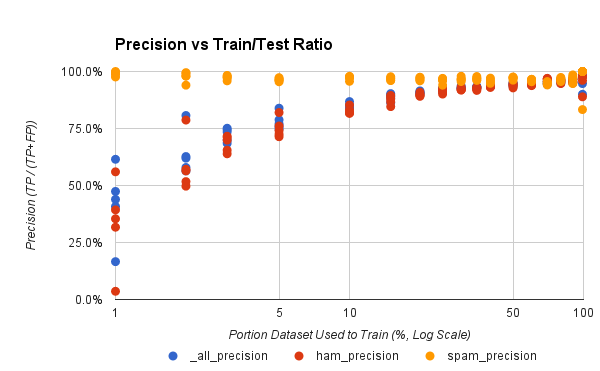
\includegraphics[width=90mm]{img/sms_basic-precision.png}
    \caption{Overall, spam-specific, and ham-specific precisions found at varying portions of the dataset used to train}
    \label{fig:spamBasicPrecision}
\end{figure}

\begin{figure}[ht!]
    \centering
    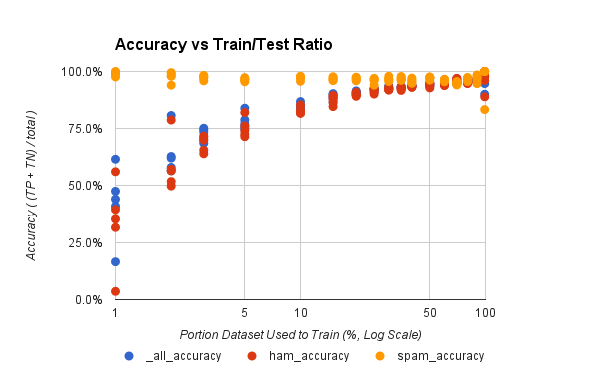
\includegraphics[width=90mm]{img/sms_basic-accuracy.png}
    \caption{Overall, spam-specific, and ham-specific accuracies found at varying portions of the dataset used to train}
    \label{fig:smsBasicAccuracy}
\end{figure}

\begin{table}
    \begin{tabular}{rrrrrrrr}
        \hline
        \textbf{Train} &
        \textbf{\begin{math}P_{All}\end{math}} & \textbf{\begin{math}P_{Ham}\end{math}} & \textbf{\begin{math}P_{Spam}\end{math}} &
        \textbf{\begin{math}A_{All}\end{math}} & \textbf{\begin{math}A_{Ham}\end{math}} & \textbf{\begin{math}A_{Spam}\end{math}} &
        \textbf{t} \\ [0.5ex]
        \hline\hline
        1\%  & 99.1 & 99.1 & 99.0 & 99.1 & 99.1 & 99.0 & 62s \\
        5\%  & 99.7 & 99.8 & 99.4 & 99.7 & 99.8 & 99.4 & 58s \\
        15\% & 99.9 & 99.9 & 99.6 & 99.9 & 99.9 & 99.6 & 64s \\
        \hline
    \end{tabular}
    \caption{Mean \% precision (P) and accuracy (A) found over 1000 iterations at a number of train/test ratios,
    and the time (t) to split and evaluate each}
    \label{table:smsBasicResults}
\end{table}


\subsection{Extending the Classifier}
\label{subsection:advancedResults}
TODO
